\documentclass[dvipdfmx, border=10pt]{standalone}
\usepackage{amsmath}
\usepackage{amssymb}
\usepackage{tikz-cd}

\newcommand{\mor}{\mathrm{Mor}}
\newcommand{\calA}{\mathcal{A}}
\newcommand{\morcalA}{\mor_{\calA}}
\newcommand{\morcalAd}{\mor_{\calA'}}

\begin{document}
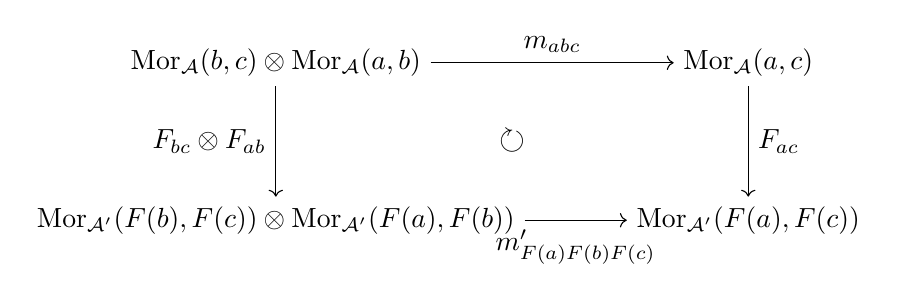
\begin{tikzpicture}[commutative diagrams/every diagram]
  \node (TL) at (0, 2) {$\morcalA(b,c) \otimes \morcalA(a,b)$};
  \node (TR) at (6, 2) {$\morcalA(a,c)$};
  \node (BL) at (0, 0) {$\morcalAd(F(b), F(c)) \otimes \morcalAd(F(a),F(b))$};
  \node (BR) at (6, 0) {$\morcalAd(F(a),F(c))$};
  \path[->] (TL) edge node[above] {$m_{abc}$} (TR);
  \path[->] (TL) edge node[left]  {$F_{bc} \otimes F_{ab}$} (BL);
  \path[->] (TR) edge node[right] {$F_{ac}$} (BR);
  \path[->] (BL) edge node[below] {$m'_{F(a)F(b)F(c)}$} (BR);
  \node at (3, 1) {\large $\circlearrowright$};
\end{tikzpicture}
\end{document}